\documentclass[11pt]{article}

\usepackage{latexsym}
\usepackage{amsmath}
\usepackage{amssymb}
\usepackage{amsthm}
\usepackage{graphicx}
\usepackage{wrapfig}
\usepackage{pseudocode}
\usepackage{url}
\usepackage[backref, colorlinks=true, citecolor=red, urlcolor=blue, pdfauthor={Jyh-Ming Lien}]{hyperref}


\newcommand{\handout}[5]{
  \noindent
  \begin{center}
  \framebox{
    \vbox{
      \hbox to 5.78in { {\bf Advanced Algorithms} \hfill #2 }
      \vspace{4mm}
      \hbox to 5.78in { {\Large \hfill #5  \hfill} }
      \vspace{2mm}
      \hbox to 5.78in { {\em #3 \hfill #4} }
    }
  }
  \end{center}
  \vspace*{4mm}
}

\newcommand{\lecture}[4]{\handout{#1}{#2}{#3}{}{#1}}

\newtheorem{theorem}{Theorem}
\newtheorem{corollary}[theorem]{Corollary}
\newtheorem{lemma}[theorem]{Lemma}
\newtheorem{observation}[theorem]{Observation}
\newtheorem{proposition}[theorem]{Proposition}
\newtheorem{definition}[theorem]{Definition}
\newtheorem{claim}[theorem]{Claim}
\newtheorem{fact}[theorem]{Fact}
\newtheorem{assumption}[theorem]{Assumption}

% 1-inch margins, from fullpage.sty by H.Partl, Version 2, Dec. 15, 1988.
\topmargin 0pt
\advance \topmargin by -\headheight
\advance \topmargin by -\headsep
\textheight 8.9in
\oddsidemargin 0pt
\evensidemargin \oddsidemargin
\marginparwidth 0.5in
\textwidth 6.5in

\parindent 0in
\parskip 1.5ex
%\renewcommand{\baselinestretch}{1.25}

\begin{document}

\lecture{Program Assignment 1}{Fall 2015}{Prof.\ Jyh-Ming Lien}{---}

152cpg04 \quad  Yunjoo Park

\href{mailto:yunjoopark12@gmail.com}{\it yunjoopark12@gmail.com}

git clone \href{https://github.com/yunjoopark/programmingAssignment1.git}{https://github.com/yunjoopark/programmingAssignment1.git}


\section{3D Delaunay Triangulation}

\subsection{Problem definition and Analysis}
Let  $P := \{p_1,p_2,...,p_n\}$ be a set of points in the plane. In that, a \textit{triangulation} of $P$ is defined a maximal planar subdivision whose vertex set is $P$ and it denoted by $DT(P)$. if there are three points $p_i,p_j,p_k \in P$ are vertices in the same face of the $DT(P)$, the circle through $p_i,p_j,p_k$ contains no other points. This circle is called the circumcircle of the triangle defined by $(p_i,p_j,p_k)$. We can relatively easily compute the \textit{Delaunay Triangulate} by using convex hull( ``\href{http://www.qhull.org/}{qhull}").
In this report, 3D points are given. Lift the points to 4D so that each point is $(x, y, z, x^2+y^2+z^2)$ and compute the convex hull in 4D. As a result, we could get the tetrahedron as the ouput. 

\subsection{Platforms}
Languages: C

Platform: Microsoft visual Studio 2013

\subsection{Examples of Inputs}


\begin{figure}[h]
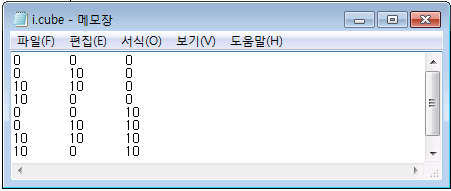
\includegraphics[width=.5\textwidth]{FIGS/inputs}
\centering
\caption{An Example of inputs}
\end{figure}

1. There are 11 test data.

2. Each data file has different values.

3. Each line has three value, $x, y, z$.

\clearpage

\subsection{Problem-solving methods and algorithms}

For lifting the given 3D points to 4D, add another $pt4 = x^2 + y^2 + z^2$. Then, we have the points in 4D. Next, compute convex hull in 4D by using qhull. Since this is in 4D, each face is a tetrahedron. Therefore, we have to call a \textit{function MakeNullTetra()}. For each tetra, we have check its volume with a \textit{function Volumei(face, vertex)}. Make a triangle with any three points in tetra and let the other point be a vertex. Except a tetrahedra having volume $0$, make the facet. Then, we could get the Delaunay Triangulation with the set $P$.

\subsection{Results Analysis and Discussion}
In this report, render a delaunay triangulation graph from given 3D points. I could study the concept the Delaunay Triangulation. Firstly, speaking about the Delaunay Triangulation, it could be computed by convex hull. For reporting triangles as a result, I have to confirm whether a trinagle is facing down or not. The normal of a tetra has 4 values becasue the given points is 3D. Among them, if the tetra is lower facet, the last coefficient of its normal is clearly negative. 
Thus, I can confirm which is lower facet by comparing \textit{normal} with $0.0$. Also, I have to check the volume of tetra because there could be a tetra having no the volume. Make faces only meeting two conditions mentioned. Since using \textit{qhull}, the algorithms has the time complexity $O(nlogn)$.
Actually, I tried to complete this project with a macOS. I however, spent much of my time to fix a problem about the qhull libarary. I downloaded it and copied it to the qhull directory. But, the GUI Keys did not work. So, I completed the project in Windows. Also, I think it was a very good opportunity to learn the \LaTeX and \textit{git}. I think they are important in my study.

\clearpage

\subsection{Outputs}
\begin{figure}[h]
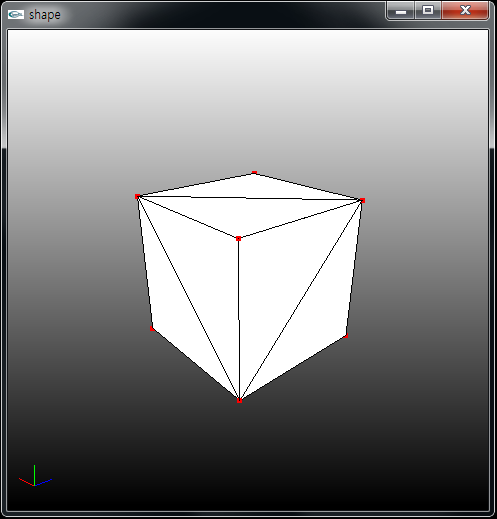
\includegraphics[width=.5\textwidth]{FIGS/icube-faces}
\hspace{1cm}
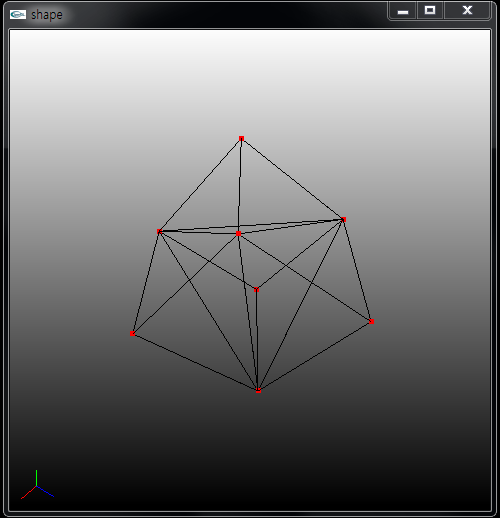
\includegraphics[width=.5\textwidth]{FIGS/icube-edges}

\caption{facets and edges \textit{i.cube}}
\end{figure}

\begin{figure}
\vspace{1cm}
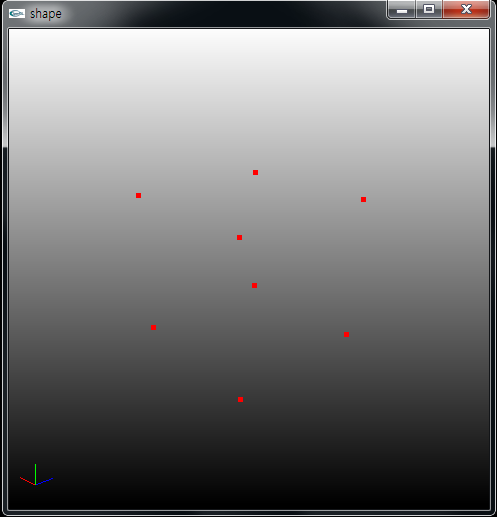
\includegraphics[width=.5\textwidth]{FIGS/icube-vertices}
\hspace{1cm}
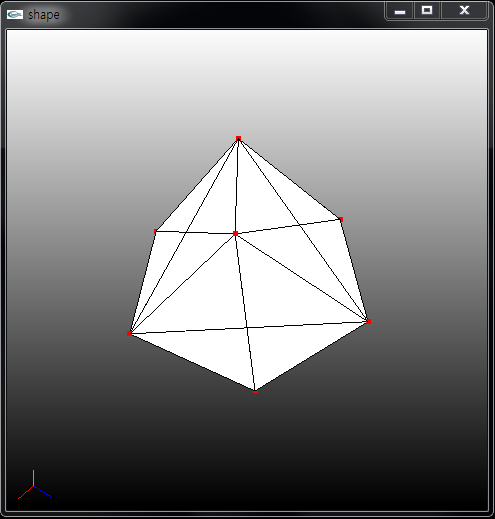
\includegraphics[width=.5\textwidth]{FIGS/icube-tetra}
\caption{vertices and tetrahedra \textit{i.cube}}
\end{figure}

\begin{figure}[h]
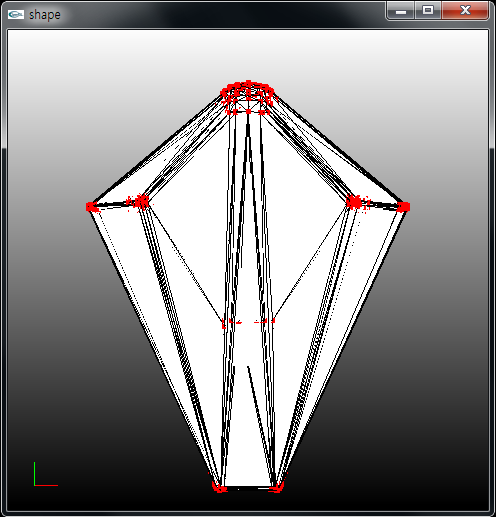
\includegraphics[width=.5\textwidth]{FIGS/ibb-tetra}
\hspace{1cm}
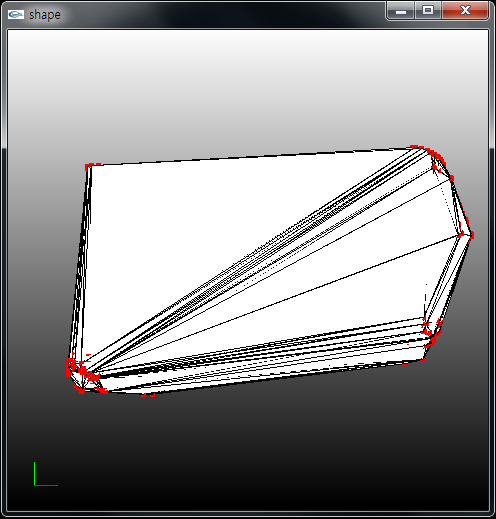
\includegraphics[width=.5\textwidth]{FIGS/ibull-tetra}
\caption{tetrahedra \textit{i.bb and i.bull}}
\end{figure}

\begin{figure}[h]
\vspace{1cm}
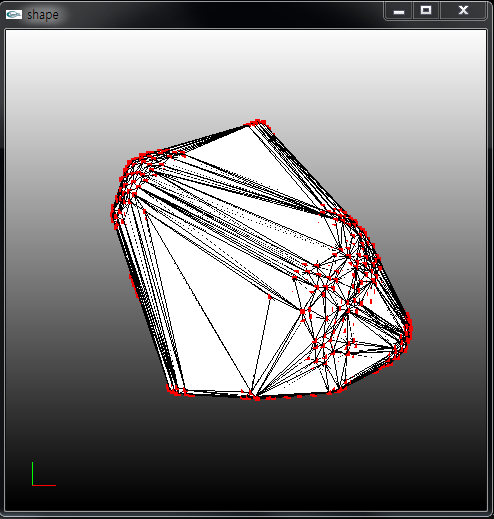
\includegraphics[width=.5\textwidth]{FIGS/ibunny-tetra}
\hspace{1cm}
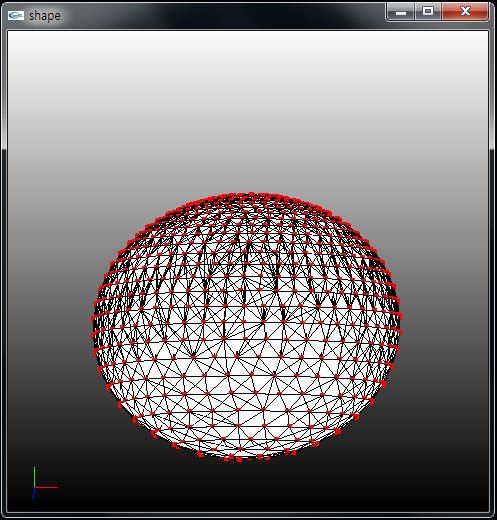
\includegraphics[width=.5\textwidth]{FIGS/iellipsoid-tetra}
\caption{tetrahedra \textit{i.bunny and i.ellippsoid}}
\end{figure}

\begin{figure}[h]
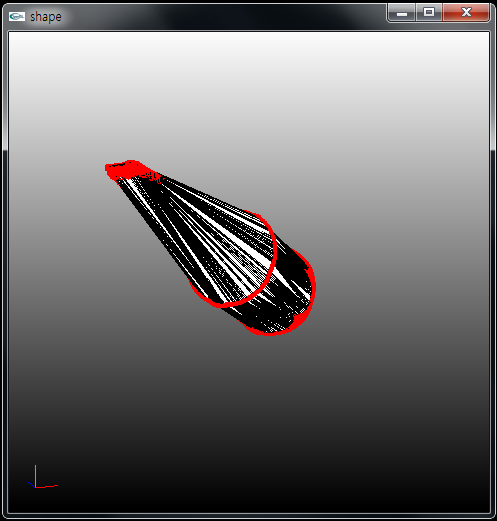
\includegraphics[width=.5\textwidth]{FIGS/iscrewdriver-tetra}
\hspace{1cm}
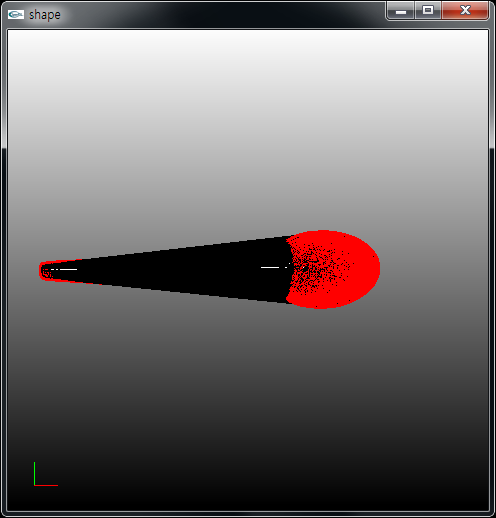
\includegraphics[width=.5\textwidth]{FIGS/ispoon-tetra}
\caption{tetrahedra \textit{i.screwdriver and i.teeth}}
\end{figure}

\begin{figure}[h]
\vspace{1cm}
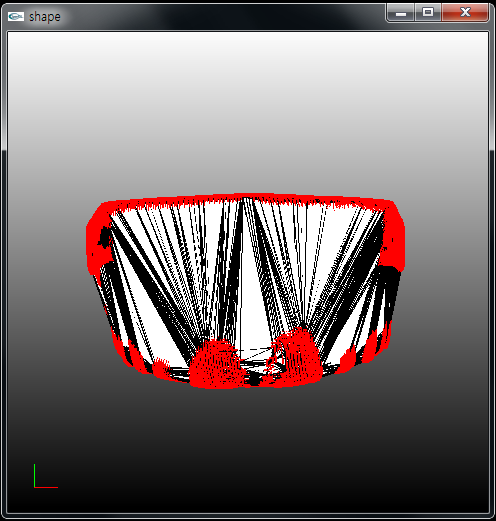
\includegraphics[width=.5\textwidth]{FIGS/iteeth-tetra}
\hspace{1cm}
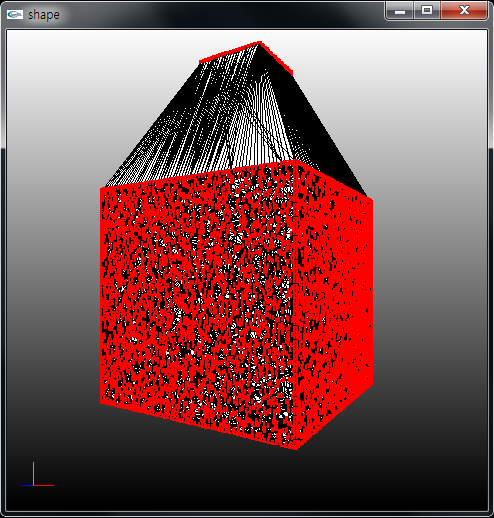
\includegraphics[width=.5\textwidth]{FIGS/iT-tetra}
\caption{tetrahedra \textit{i.T and i.ellippsoid}}
\end{figure}

\begin{figure}[h]
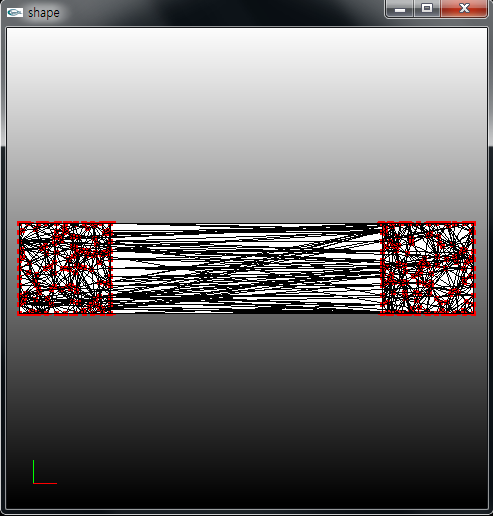
\includegraphics[width=.5\textwidth]{FIGS/iU-tetra}
\hspace{1cm}
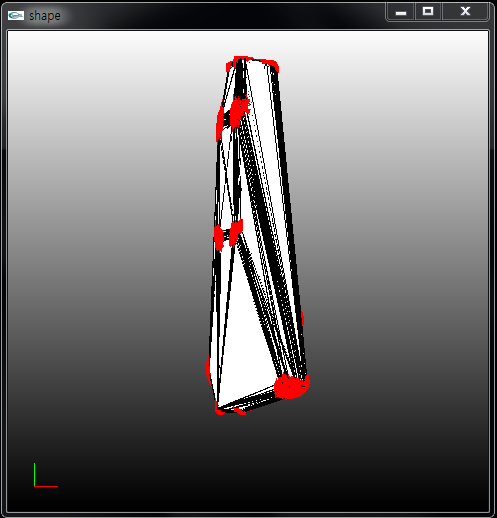
\includegraphics[width=.5\textwidth]{FIGS/iwoman-tetra}
\caption{tetrahedra \textit{i.U and i.woman}}
\end{figure}


\end{document}


